\section{Introduction}

In software engineering, finding a mapping of elements from a language to another is a very common task. Modern programs depend on lots of library APIs, when those APIs change, usually many locations of the client programs need to be changed. Usually, APIs libraries are implemented and maintained in multiple languages. Taking an example with Lucene, a popular search engine, Lucene provides APIs that allows a third party client to access to its core features, thus there are a lot of Lucene clients that implemented in multiple languages such as Java, C\#, Python, etc. Lucene is originally implemented in Java, as a result, the Java client of Lucene is the version that needs to be evolved and maintained first, then the others come later. Thus the developer usually needs to keep an eye on the Java client while implementing another client, such as C\#, in order to synchronize the code of the clients. Because of such reason, there is a need for an approach to find a mapping between different languages, not only for the code structure but also for the semantics of the code.

Distributed word representations can be learned from the distributional patterns in corpora. In the past, such representations can be constructed by counting co-occurrences, so that the features in one word's representation corresponded to other words. Word2vec (Mikolov et al., 2013) \cite{mikolov2013distributed}, which is a neural-based language model, is an alternative method for learning vector representation of words, aka \textbf{embedding}. It uses language data to capture latent semantic features with respect to language modeling objective. The objective can be either to predict the context given a word or predict a word given a context. The representation learned by neural network models perform effectively in tackling various NLP tasks such as sentiment analysis, sentence parsing and neural machine translation (NMT).

Recently, NMT models have emerged as an alternative to statistical, phrase-based translation models, and achieved impressive translation performance. The objective of NMT is to generate an appropriate sentence in a target language T given a sentence in the source language S. The NMT system first aggregates the embedding of each word in the sentence through an encoder to build a "thought" vector, which is a sequence of number to represent the sentence meaning. and a decoder, then, processes the sentence vector to produce a translation. It raises a question: "\textbf{\textit{Can we build a NMT model for programming languages?}}". We have seen that at character-level, the neural network model is capable of writing Linux kernel after learning the entire Linux-based source code, as described in \cite{Karpathy}. Thus the neural-based technique to generate source code is an achievable target.

Inspired by both of these, in this paper, we aim to find useful mappings between languages by learning a shared token embeddings. To the best of our knowledge, we are the first to use a \textbf{neural-based \textit{programming language model}} to learn a \textbf{\textit{share embeddings cross-lingually}}. By learning a \textbf{cross-lingual shared embedding space}, mapping similar elements between languages is achievable, thus this can be served as a foundation of NMT for programming languages. In our evaluations, we demonstrate the empirical strength of our model to represent a code fragment effectively for code clone detection task. We also show that by adding semantic keywords into the source code in the normalizing step, we can map the components of two languages accurately. 

\section{Background}

\subsection{Background on Word2Vec}

Word2vec is a group of related models that are used to produce word embeddings. These models are shallow, two-layer neural networks that are trained to reconstruct linguistic contexts of words. Word2vec takes as its input a large corpus of text and produces a vector space, typically of several hundred dimensions, with each unique word in the corpus being assigned a corresponding vector in the space. Word vectors are positioned in the vector space such that words that share common contexts in the corpus are located in close proximity to one another in the space. Mikolov et al.\cite{mikolov2013distributed} introduce two variances of Word2Vec, which are Continuous Bag-of-Words (CBOW) and skip-gram. We show skip-gram model in Figure 1 as we use it in our work.

\subsubsection{The skip-gram model}
The training objective of the skip-gram model is to find word representations that are useful for predicting the surrounding words in a sentence or a document. In other words, The skip-gram model aims to predict the word given the contexts. More formally, given a sequence of training words w1, w2, w3, . . . , wT , The basic skip-gram formulation defines \begin{math}p(w_{i+j} | w_{t})\end{math} using the softmax function:

\begin{displaymath}
p(w_{O}|w_{I}) = \frac{exp({{v'}_{w_{O}}}^{T}v_{w_{I}})}    {\sum_{w=1}^W exp({{v'}_{w}}^{T}v_{w_{I}})}
\end{displaymath}
where \begin{math}v_{w}\end{math} and \begin{math}{v'}_{w}\end{math} are the “input” and “output” vector representations of w, and W is the number of words in the vocabulary.

As described in (Mikolov at at.; 2013)\cite{mikolov2013distributed}, the skip-gram model (works well with small amount of the training data, represents well even rare words or phrases, while the Continuos Bag of Words model (CBOW) is several times faster to train than the skip-gram and slightly better accuracy for the frequent words. Since CBOW considers one target word and many context words, the task here is to predicting the word given its context, it needs a bigger dataset to train for target vectors compared to datasets used in skip-gram. In other words, a dataset with short sentences but with high number of samples is suitable for the CBOW model. On the other hand, the skip-gram model is designed to predict the context, so it needs a dataset with long sentences and low number of samples due to many target words for single context word. In our case, a file (.java or .cs) are usually quite long, compare to a normal sentence in Natural language, then the skip-gram is a more suitable model in this case. 


\subsubsection{ Parameters of the skip-gram model}
Here we want to give a brief explanation about the parameters that are being used for training with our data set.
\begin{description}
	\item [$\bullet$] \textbf{Negative sampling}: Training a neural network means taking a training example and adjusting all of the neuron weights slightly so that it predicts that training sample more accurately. In other words, each training sample will tweak all of the weights in the neural network. The size of the vocabulary means that our skip-gram neural network has a tremendous number of weights, all of which would be updated slightly by every one of our large number of training samples. Instead of taking the probability of the context word compared to all of the possible context words in the vocabulary, this method randomly samples 2-20 possible context words and evaluates the probability only from these. In other words, negative sampling addresses this by having each training sample only modify a small percentage of the weights, rather than all of them.
	
	\item [$\bullet$] \textbf{Subsampling rate}: In a nutshell, subsampling is a method of diluting very frequent words, akin to removing stop-words. The subsampling method presented in (Mikolov et al., 2013) \cite{mikolov2013distributed} randomly removes words that are more frequent than some threshold \textit{t} with a probability of \textit{p}.
	
	\item [$\bullet$] \textbf{Window size}: The window size is randomly chosen between 1 and max size for each training sample, resulting in words with the maximum distance being observed with a probability of 1/c while words directly next to the given word are always observed. For example, if the window is set to 5 then for the current word w surrounding 10 words will be taken as context words.
	
\end{description}

\begin{figure}[t!]
	
	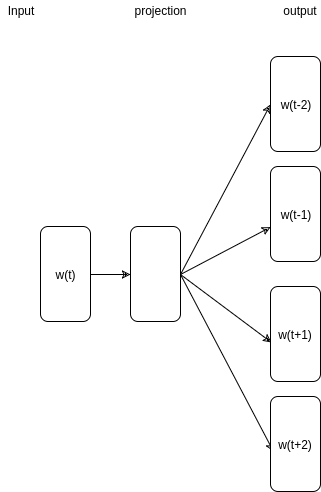
\includegraphics[width=0.20\textwidth]{skipgram}
	\caption{The Skip-gram model architecture. The training objective is to learn word vector representations that are good at predicting the nearby words.}
	\label{fig:clf}
\end{figure}

\section{Our Approach}
\subsection{Overview}

\begin{figure*}[t!]
	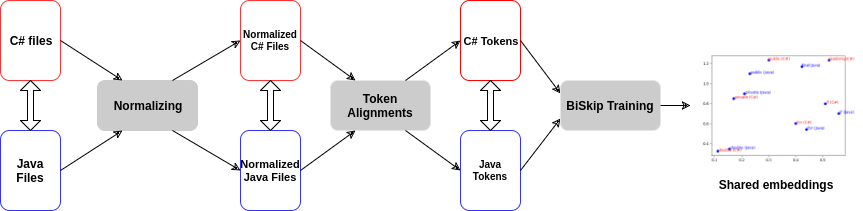
\includegraphics[width=0.60\textwidth]{approach}
	\caption{An overview of our framework}
	\label{fig:clf}
\end{figure*}



Figure 2 is the overview of our approach. There are 4 steps:
\begin{description}
    \item [$\bullet$] \textbf{Files alignment}: Collect data cross-lingually and get the aligned files. The process to get the aligned files are shown in section 4.1.
	\item [$\bullet$]\textbf{Data Normalizing}: This is the key step to get a better shared embedding by adding more semantic meanings to the training data. This step is comprised of 3 steps: preprocessing, adding semantic information and postprocessing the data.
	\item [$\bullet$] \textbf{Token Alignment}: Before learning the shared embeddings cross-lingually, we need to get the token alignment information. In our case, we do not have the monotinic token alignments. In addition, not like the natural language, the tokens in a programming language can be anything, except some language keywords, e.g: \texttt{if, for, while, public}, etc. So we utilized existing unsupervised token alignment techniques proposed by Liang \cite{liang2006alignment}.
	\item [$\bullet$] \textbf{BiSkip Training}: Once we get the token alignments information, we use it to learn shared embedding for all tokens in both languages.
\end{description}




\subsection{Data Normalizing}

In Natural Language Processing, the data normalizing step is a process to remove uninteresting contents from the data set and transform the rest into normalized comparison units. In our case, we are performing Programming Language Processing, besides removing uninteresting contents, we add more semantic features into training corpus with the first intuition that these features are able to maximize the probability of similar elements to appear together in the same context, the second intuition is to remove the syntactic gap between languages. This is the key step to learn the embedding cross-lingually. This process involes 3 sub-processes:

\begin{description}
	\item [$\bullet$] \textbf{Pre-processing}: We remove all of the useless information such as comments out source code, special character, but not all of them. In order to keep as many semantic meanings as we can, we treat the operators as tokens that also need to learn the embeddings. Usually, the operators will be similar to the special character, to distinguish between them, we adopt Srcml \cite{collard2011lightweight} to parse the source code, so we can identify if a token is a language operator or just a special character
	\item [$\bullet$] \textbf{Adding semantic information}: Once we get the XML representation of the source code, we have the information of each element from the codes, we traverse the XML representation to add or replace code elements with predefined keywords to add more semantic meaning to the raw source code. We selectively present some of the rules to add or replace code elements with keywords in Table 1.
	\item [$\bullet$] \textbf{Post-processing}: Once we get the enhanced semantic version of the code, the camel case tokens and tokens with underscores are split by upper case letters and the underscore to reduce differences between programming styles.
\end{description}

\begin{figure}[t!]
	
	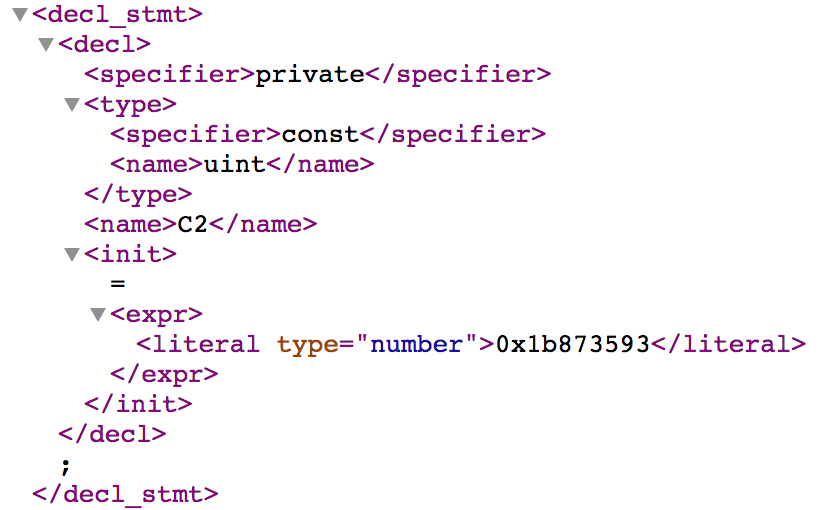
\includegraphics[width=0.30\textwidth]{srcml_sample}
	\caption{SrcML sample}
	\label{fig:clf}
\end{figure}

In Table 1, we selectively pick out some typical elements of programming languages to demonstrate our data normalizing process, the examples provided in the Table can be written either in \text{C\#} or Java. Taking an example, we have the code fragment: \texttt{for(int i = 0; i $<$ 10; i++)}, which is a simple for loop with three elements, the initialization part, the condition part and the afterthought part. We apply rule 5 into the initialization part, which transforms the variable \textbf{i} into the fixed keyword \textbf{identifier}. Then we apply rule 5 and rule 8 to the condition part, by transforming \textbf{i} into \textbf{identifier} and \textbf{10} to \textbf{literal\_type number}. Finally, we apply rule 13, rule 9 to add the keyword \textbf{operator} before \textbf{++}. 

\begin{table*}
	
	\label{tab:freq}
	\resizebox{\textwidth}{!}{
	\begin{tabular}{p{2cm}|p{0.7cm}|p{2cm}|p{3cm}|p{4cm}|p{4cm}}
	
		\hline
		\textbf{Element}&\textbf{Index} &\textbf{Sub-Element}&\textbf{Rule}&\textbf{Example code}&\textbf{Applied Rules}\\
		
		\hline
		Statements & 1&if statement & add \textbf{condition} & \texttt{if(x$>$5) y+=4} & if expr type int identifier operator $>$ literal\_type number expr\_stmt expr identifier operator += literal\_type number\\\cline{2-6}
		
		&2& for statement & add \textbf{condition}, \textbf{control} & \texttt{for(int i=0;i$<$10;i++)}  & for control init type int idenfier operator = number condition expr identifier operator $<$ literal\_type number identifier operator ++\\\cline{2-6}
		
		&......&&&& \\\cline{2-6}
		
		\hline
		Expressions &3& function call & add \textbf{call} & \texttt{Console.WriteLine("out")}  & expr\_stmt expr call Console Write Line argument literal\_type string\\\cline{2-6}
		
		&......&&&& \\\cline{2-6}
		
		\hline
		Declarations, Definitions and Initializations &4& variable declaration statement& add \textbf{decl\_stmt} & \texttt{int i} & decl\_stmt decl type int identifier\\\cline{2-6}
		
		&5& variable identifier definition & replace with \textbf{identifier} & \texttt{string s}& string identifier\\\cline{2-6}

		&6& function declaration & add \textbf{function\_decl} & \texttt{void doWork()}& function\_decl void do Work \\\cline{2-6}
		&......&&&& \\\cline{2-6}
		\hline
		Others &7& inheritance list & add \textbf{super} & \texttt{class Foo: Bar \{ \}} & class Foo super Bar\\\cline{2-6}
		
		&8& literal & add \textbf{literal\_type} & \texttt{int x = 9}& int identifier operator = literal\_type number \\\cline{2-6}
		
		&9& operator & add \textbf{operator} & \texttt{a \& b }&  identifier operator \& identifier \\\cline{2-6}
		&......&&&& \\\cline{2-6}
	
	
		\hline
	\end{tabular}}
	\medskip
	\caption{Source code Transformation Rules.}
\end{table*}
\subsection{ Unsupervised token alignment}

Once we finish normalizing our training data, we want to learn a shared embedding space between tokens crosslingually rather than just monolingually. In order to do that, we need to obtain aligned information from such languages. We do not have the alignment information, thus the alignment information must be obtained under the unsupervised manner. We briefly review the sequence-based unsupervised token alignment models. Generally, the token alignment model are generative models of the form p(\textbf{t $|$ s}) = $\displaystyle\sum_{a} p(\textbf{a,t $|$ s})$, where $\textbf{s} = (s_{1},..., s_{J})$ is the source sentence, $\textbf{t} = (t_{1},..., s_{J})$ is the target sentence and $\textbf{a} = (a_{1},..., a_{J})$ is the asymmetric alignment which specifies the position of a token in source language aligned to each target language. Bekerley aligner (Liang et al. \cite{liang2006alignment}) is a joint training approach, while the source language and target language play a symmetric role in the word alignment task, sequence-based models are asymmetric,they are generative models of the form p(\textbf{t $|$ s})(S $\rightarrow$ T) or p(\textbf{s $|$ t})(T $\rightarrow$ S) by reversing the roles of source and target. This suggests that two models make different types of errors that can be eleminated upon intersection. Figure 4 shows an example alignment of tokens of code fragments between \text{C\#} and Java code as an output of the Bekerley aligner.

\begin{figure}[t!]
	
	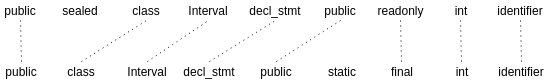
\includegraphics[width=0.48\textwidth]{alignment}
	\caption{Sample alignment of code fragments between \text{C\#} and Java code, both the fragments have already been normialized.}
	\label{fig:clf}
\end{figure}

\subsection{The Billingual Skipgram Model}

Once we get the token alignment information, we want to learn the shared embedding space for tokens from both languages. We use the billingual skip gram model (BiSkip) \cite{luong2015bilingual} to learn this space. The motivation behind the BiSkip is to learn a shared embedding space between tokens cross-lingually rather than just monolingually. Rather than just predicting the tokens in the source language, they use the tokens in the source language to additionally predict their aligned tokens in the target languages. Imagine that if we know that the token \textit{readonly} in \text{C\#} is aligned to and has the same meaning as the token \textit{final} in Java in Figure 5, we can simply substitute \textit{readonly} and use \textit{final} to predict the surrounding tokens such as \textit{int} and \textit{public}. 

Given an alignment link between a token $t_{1}$ in a language $l_{1}$ and a token $t_{2}$ in another language $l_{2}$, the BiSkip model uses the token $t_{1}$ to predict the surrounding tokens of the token $t_{2}$ and vice versa. We can think of this BiSkip model as training four skipgram models jointly which predict tokens betwwen the follow pairs of languages: $l_{1} \rightarrow l_{1}, l_{2} \rightarrow l_{2}, l_{1} \rightarrow l_{2}, l_{2} \rightarrow l_{1}$.



\begin{figure}[t!]
	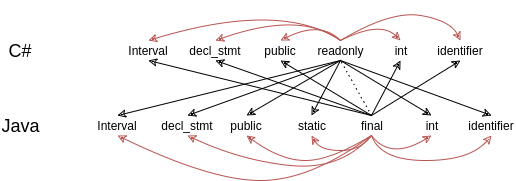
\includegraphics[width=0.35\textwidth]{biskip_align}
	\caption{Billingual Skipgram Model - besides predicting within languages, the model also predict crosslingually based on the alignment information \text{C\#} and Java}
	\label{fig:clf}
\end{figure}

\section{Experiments}


\subsection{Data}
We collect data from 10 open source projects cross-lingually in C\# and Java. With the intuition that the different implementations of the same project in different languages contains the same logical information, thus files with the same indicator also contain the same logical information, so they are aligned to each other. In natural language processing, such information is called aligned sentences or aligned documents. Here we call them aligned files. Taking Lucene as an example, the file \texttt{AbstractEncoder.cs} under C\# Lucence Client project has the same indicator \texttt{AbstractEncoder} with the file \texttt{AbstractEncoder.java} under Java Lucene Client project, so they are aligned to each other. We get around 13770 pairs of aligned implementation over 10 projects and we normalize all the pairs. Table 2 is an overview of our training data set.

\begin{table*}
	
	\label{tab:freq}
	\resizebox{\textwidth}{!}{
		\begin{tabular}{c|cc|cc|cc|cc|cc|cc|cc|cc|cc|cc}    
			\hline
			Projects&
			\multicolumn{2}{c}{aws-sdk} &
			\multicolumn{2}{c}{antlr} & \multicolumn{2}{c}{datasax} & \multicolumn{2}{c}{factual} & \multicolumn{2}{c}{fpml} & \multicolumn{2}{c}{log4j/4net} & \multicolumn{2}{c}{lucene} & \multicolumn{2}{c}{spring} & \multicolumn{2}{c}{zeromq} & \multicolumn{2}{c}{mongodb}  \\
			\hline
			Languages&C\# & Java&C\# & Java &C\# & Java &C\# & Java &C\# & Java &C\# & Java &C\# & Java &C\# & Java &C\# & Java &C\# & Java \\
			\hline
			Files& 18801 & 23503 & 593 & 351  & 545 & 548 & 55 & 63 & 124 & 124 &293 & 298 & 2709 & 5703 & 2364 & 5697 & 206 & 220 & 1914 & 1087 \\
			\hline
			Aligned files& \multicolumn{2}{c|}{9850}&\multicolumn{2}{c|}{205} & \multicolumn{2}{c|}{98}  & \multicolumn{2}{c|}{35} & \multicolumn{2}{c|}{140} & \multicolumn{2}{c|}{78} & \multicolumn{2}{c|}{2445} & \multicolumn{2}{c|}{550} & \multicolumn{2}{c|}{89} & \multicolumn{2}{c}{280} \\
	\end{tabular}}
	\caption{Overview of our training data set}
\end{table*}

\subsection{Training}
We use the following settings: stochastic gradient descent with a default learning rate 0.025, negative sampling with 30 samples, skip-gram with context window of size 10, and a subsampling rate of value 1e-4. All models are trained for 10 epochs and the learning rate is decayed to 0 once training is done. In Natural Language, according to \cite{pennington2014glove}, the number of words is usually large in the training set and we need a large dimension (range from 100 to 300) to capture the whole semantic meaning of the words. In our case, our training set is relatively smaller, so we choose 50 as the dimension size.
\subsection{Evaluation Tasks}
We evaluate our architectures on 3 tasks: tokens matching, elements matching and clone detection. These 3 tasks represent for different granularity of the source code. Here we want to evaluate the effectiveness of our approach when mapping elements in different granularity cross-lingually. In the tokens matching task, we want to evaluate how effective our model is on the token level, mapping at this level is important because this is served as a based level for a more high-level representation of source code. The elements matching task represent a more coarse-grained level of source code. Formally, an element, such as expression, declaration or statement is a combination of tokens in a structural way. Finally, we evaluate our approach by comparing the similarity of some "big" code fragments. We use the diff data set from \cite{cheng2017clcminer}, which contains the code hunk from the revision history, so called \textit{diff}. These may not a complete code fragment but still, contain some structural and semantic meaning.
\subsubsection{Tokens matching}
This task measures the semantic quality of the learned token vectors cross-lingually.  We manually defined the token-level alignment list between languages'as the ground truth. The types of tokens to be considered are the language keywords and the operator symbols (such as \&\&,$+$,$+=$, etc). For example, \textbf{\textit{readonly(C\#)}} should be aligned to \textbf{\textit{final(Java)}}. Then for each C\# keyword in the list, we take out the vector representation of that keyword in the C\# vector space, we use that keyword as the query to find k-nearest neighbors of that key word in the Java vector space based on Euclidean distance, we do this task in both directions, from C\# to Java, and from Java to C\#. 

Once we get the results, we calculate the Average Precision of that query. 
The Average Precision can be calculated as follow:
\begin{displaymath}
AP = \frac{\prod_\text{k=1}^n P(k)*rel(k)}{d}
\end{displaymath}
where P(k) is the precision at cut-off k in the list, rel(k) is an indicator function equaling 1 if the item at rank k is a relevant document, zero otherwise and d is the number of relevant documents.

Once we get the AP for each query, we then calculate the Mean Average Precision for all queries. The MAP can be calculated as follow:
\begin{displaymath}
AP = \frac{\prod_\text{p=1}^Q AP(q)}{Q}
\end{displaymath}
where q is the query, and Q is the number of total queries.

\subsubsection{Elements Matching}
In this task, we want to measure the semantic quality of the learned token vectors cross lingually. In software engineering, expressions, definitions, declarations, and statements are basic elements to constitute complicated functionality of a program. We want to evaluate how we can match such elements between different languages together. For example, \textbf{public interface AnotherScopeTestInterface\{\}} in Java and \textbf{public interface IAttributeRenderer \{\}} in C\# are definitely defined in different context with different usage, but they both means to declare an interface, it should not be mixed up with any other declarations, e.g variable declaration, class declaration, etc. For each type of elements, we define sub-elements of that type. For each sub-element, we randomly extract code fragments from real software projects in both languages. For each code fragment, we calculate the vector representation of it and we take the vector representation of code fragment from the source language as the query to rank the most similar code fragments in the same group of the target language based on Euclidean distance. We use the Mean Reciprocal Rank (MRR), which is a statistic measure for evaluating a process that produces a list of possible responses to a sample of queries, to evaluate our matching process.

The MRR metric can be calculated as follow:
\begin{displaymath}
MRR = \frac{1}{|Q|}\sum_{i=1}^{|Q|}\frac{1}{rank_{i}}
\end{displaymath}
where i refers to the rank position of the first relevant document for the i-th query and Q is the total number of queries.

\subsubsection{Clone detection}
To evaluate the impact of our model on real world tasks, we apply our approach into the diff dataset from (Cheng at al., 2016)\cite{cheng2017clcminer} for clone detection. The dataset contains 2000 pairs of diff, one diff is from C\# and the other is from Java, each pair has been labeled either cloned or non-cloned. 

For each diff, we perform normalizing step (Section 3.1) to get the normalized version of the diff, here we call it as "token stream". Then we get the vector representation of the token stream by the averaging token vectors for all tokens in the stream, once we get the vector representation, we calculate the similarity between vectors by using the cosine similarity metric. We plot the probability (Figure 5) mass function (PMF) of a distribution of cosine similarity for all pairs of diff. Here we want to find the decision boundary to separate the 2 groups: cloned and none-cloned. 

\subsection{Result}
\subsubsection{Tokens Matching}
Each token in our model is represented by a 50 dimensional vector. To visualize our model, here we use t-Distributed Neighbor Embedding (t-SNE)\cite{maaten2008visualizing}, a technique for dimensionality reduction that is particulary well suited for the visualization of high-dimensional datasets. Figure 5 shows a visualization of shared embedding for some similar tokens between C\# and Java, each pair of similar tokens are close together, e.g \textit{\textbf{if (\text{C\#})}} should be closest to \textit{\textbf{if (Java)}} and clusters with similar functionality should be located close to each other than other clusters, e.g the \textit{\textbf{if}} cluster should be closer to the \textit{\textbf{for}} cluster because both \textit{\textbf{if}} and \textit{\textbf{for}} are control statement.

\begin{figure}[t!]
	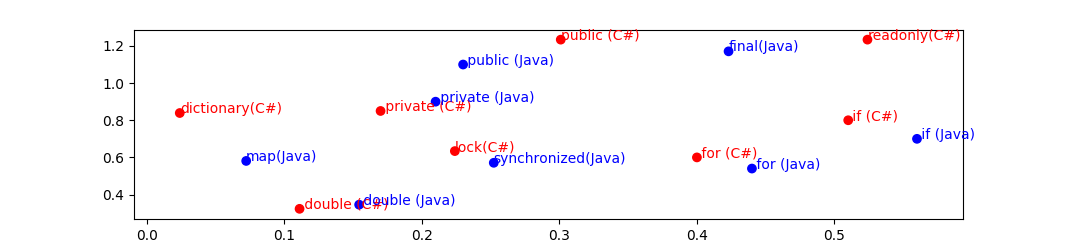
\includegraphics[width=0.45\textwidth]{example_bi2vec_tsne}
	\caption{A visualization of shared embeddings between \text{C\#} and Java.}
	\label{fig:clf}
\end{figure}

Table 2 shows some example of top 5 most similar tokens once we take a token in the source language and find the most similar tokens in the target language, we demonstrate with some tokens that are supposed to be similar in billingual languages.
\begin{table}
	
	\label{tab:freq}
	\resizebox{\columnwidth}{!}{
		\begin{tabular}{cccc}
			
			
			\multicolumn{1}{c}{readonly(C\#)}  & \multicolumn{1}{c}{exception(Java)} & \multicolumn{1}{c}{lock(C\#)} &
			\multicolumn{1}{c}{package(Java)} \\
			\hline
			Java & C\# & Java & C\# \\
			\hline
			final & throw & lock & namespace  \\
			private & exception & synchronized & using \\
			static & throwable  & open & system \\
			extends & catch & checkpoint & sealed\\
			decl & finally & held & class\\
			
			
	\end{tabular}}
	\caption{Nearest neighbor tokens - shown are the top 5 nearest tokens when we take the vector of a word from the source vector space as the query to find the nearest neigbors in the target space, as measured by the Euclidean distance.}
	
\end{table}


Table 4 shows the result when querying for 1-nearest neighbors, 3-nearest neighbors, 5-nearest neighbors, respectively.

\begin{table}
	
	\label{tab:freq}
	
	\begin{tabular}{c|cc|cc|cc}
		
		\hline
		\multicolumn{1}{c}{}  &
		\multicolumn{2}{c}{1-NN}  &
		\multicolumn{2}{c}{3-NN}  & \multicolumn{2}{c}{5-NN} \\
		\hline
		& C\# & Java & C\# & Java & C\# & Java \\
		\hline
		MAP & 0.859 & 0.852 & 0.886 & 0.857 & 0.901 & 0.864 \\    
		
	\end{tabular}
	\caption{Mean Average Precision for different top-k queries, k = 1,3,5. }    
\end{table}
\subsubsection{Elements matching}
We start with the expression matching task first. An expression is a combination of one or more explicit values, constants, variables, operators, and functions that the programming language interprets.
We only consider the \textbf{\textit{compound case expression}} since we want to evaluate the ability to get the vector representation of a compound element. Table 7 gives the detail of expression with example code. For each expression type, we randomly pick 5 expressions of that type in both C\# and Java in the data set. Consider this expression:

\texttt{arguments == null || arguments.count == 0} . 

This expression is a composition of two sub-expressions. We calculate the average of all tokens for each sub-expression. In this case, the number of sub-expressions is 2. Then we get 2 vector representations, we average these 2 vectors to get the final representation for the expression. We take a vector representation of the expression code from the source language as the query to rank the most similar code fragments in the same group of the target language based on Euclidean distance. Table 5 shows the expression type with the code example for each type. Table 7 shows the MRR score of the expressions we use to perform the evaluation.

\begin{table}
	
	\label{tab:freq}
	\resizebox{\columnwidth}{!}{
		\begin{tabular}{c|c}
			
			\textbf{Type} & \textbf{Code example}\\
			\hline
			assignment expr & \texttt{x = a}\\
			\hline
			numeric expr & 10 + 20 \\
			\hline
			function call expr & \texttt{System.out.println("Hello World!")} \\
			\hline
			tenary operator expr& \texttt{a ? x : y}\\
			
			\hline
			member and scope access expr& \texttt{person.name}\\
			
			\hline
			bit expr & \texttt{a $<<$ 1}\\
			
			\hline
			this expr & \texttt{this.x = x}\\
			
			\hline
			logical expr & \texttt{a == null}\\
			
			
			\hline
			object creation expression & \texttt{o = new Object ()}\\
			
	\end{tabular}}
	\caption{Expression types with code example}	
\end{table}


The definition, declaration, and statement are more intricate elements, they can be a composition of multiple types of elements. We define 18 sub-elements in total for these 3 elements. We base on srcML \cite{collard2011lightweight} to define the sub-elements in each group, we only consider the sub-elements that appear in both C\# and Java. Table 7 gives detail of the element with code fragment example. For each sub-element, we randomly extract 5 code fragments from real software projects for both languages. In Table 6, we selectively show some examples of the elements we use to perform the evaluation. For each code fragment, we calculate the vector representation of it by averaging tokens vectors for all tokens in the code fragment. Then we perform the similar matching task for each group like the expression matching task; and we use the MRR score to evaluate the performance of each group.  We calculate the average MRR score for each group as we want to show a more coarse-grained result of this task, the result is shown in Table 8.


\begin{table*}
	\label{tab:freq}
	
	\begin{tabular}{p{2cm}|l|p{5cm}}
		
		\hline
		Element &Sub-Element& Code Sample\\
		\hline
		Definition & method definition & \texttt{int getArea() \{
			return width * height;
			\}}\\\cline{2-3}
		
		& class definition & \texttt{class Pair \{\}}\\\cline{2-3}
		
		& enum definition & \texttt{enum Planet \{ MERCURY, VENUS, EARTH, MARS, JUPITER, SATURN, URANUS, NEPTUNE; \}}   \\\cline{2-3}
		
		& ........ &  \\\cline{2-3}
		\hline
		
		
		Declaration & field declaration & \texttt{public static int i = 10;} \\\cline{2-3}
		
		
		& array declaration & \texttt{int[] numbers = new int[5];} \\\cline{2-3}
		
		& method declaration & \texttt{void doWork();} \\\cline{2-3}
		
		
		& ........ &  \\\cline{2-3}
		\hline
		Statement & if statement & \texttt{if ( i $>$ 0 ) \{ y = x $/$ i;\}}\\\cline{2-3}
		
		& for statement & \texttt{for(int i = 0; i < 10;i++)\{\}}\\\cline{2-3}
		& ........ & \\\cline{1-3}
		
	\end{tabular}
	\medskip
	\caption{Elements Type Example - shown are 3 types: Definition, Declaration and Statement with code example. The code can be either in C\# or Java}
\end{table*}


\begin{table*}
	
	\label{tab:freq}
	\resizebox{\textwidth}{!}{
		\begin{tabular}{c|cc|cc|cc|cc|cc|cc|cc|cc|cc}
			
			\hline
			Expression Type&\multicolumn{2}{c|}{assignment} & \multicolumn{2}{c|}{numeric} & \multicolumn{2}{c|}{function call} & \multicolumn{2}{c|}{ternary operator} & \multicolumn{2}{c|}{member and scope access} & \multicolumn{2}{c|}{bit operator} & \multicolumn{2}{c|}{this} & \multicolumn{2}{c|}{logical} & \multicolumn{2}{c|}{object creation} \\
			\hline
			Language& C\# & Java & C\# & Java & C\# & Java  & C\# & Java & C\# & Java & C\# & Java & C\# & Java  & C\# & Java & C\# & Java\\
			\hline
			MRR & 0.905 & 0.912  & 0.886 & 0.857 & 0.901 & 0.864 & 0.841 & 0.874& 0.905 & 0.83& 0.78 & 0.833 & 0.924 & 0.854& 0.911 & 0.872 & 0.899 & 0.824 \\    
			
	\end{tabular}}
	\medskip
	\caption{MRR score of Expression matching}    
\end{table*}


\begin{table}
	
	\label{tab:freq}
	\resizebox{\columnwidth}{!}{
		\begin{tabular}{c|cc|cc|cc}
			
			\hline
			Element Type&\multicolumn{2}{c|}{Definition} & \multicolumn{2}{c|}{Declaration} & \multicolumn{2}{c}{Statement} \\
			\hline
			Language& C\# & Java & C\# & Java & C\# & Java \\
			\hline
			MRR & 0.685 & 0.652  & 0.643 & 0.698 & 0.601 & 0.564 \\    
			
	\end{tabular}}
	\medskip
	\caption{MRR score of Definition, Delclaration and Statement matching}    
\end{table}


\subsubsection{Clone Detection}
Figure 6 shows the probability mass function (PMF) of cosine similarity (COSIM) for all pairs of diff. The blue curve indicates the PMF of the cloned pairs, The yellow curve is for the non-cloned pairs. The x-axis is the COSIM value. The y-axis shows the probability distribution of an x-value. The COSIM of the non-cloned pairs ranges from -0.4 to 0.8 and most of them assemble equally from 0.3 to 0.7, while the COSIM of cloned pairs ranges from 0.6 to 1 and most of them assemble equally from 0.8 to 1.

Because of this difference in COSIM distribution between cloned and non-cloned pairs, there exists a decision boundary to separate them, then this task becomes a classification problem. The COSIM is the only feature for this classification model. We use these well-known classifiers: Logistic Regression, Support Vector Machine and Random Forest to evaluate this problem. For per-project's pairs, we use 10-fold validation to evaluate the performance of the classification model.

To prove that the normalizing step provides a better representation of token, we do the same task for the "non-normalizing" version of the data set. In Table 6, there are 2 parts, the first part is the classification result when we apply the normalizing step into the training data, the second part is for the "non-normalizing" version.


\begin{figure}[t!]
	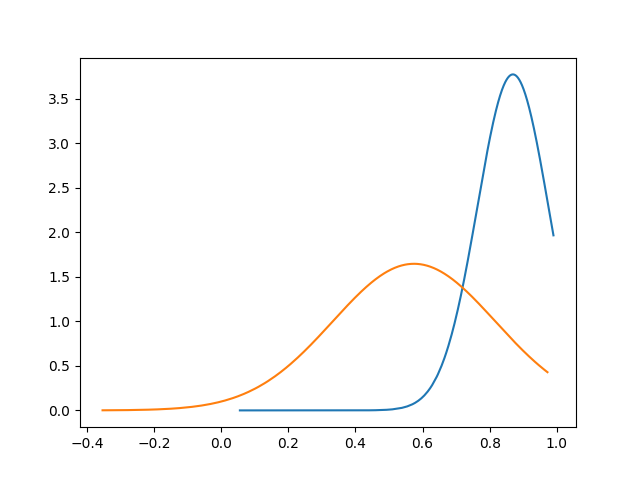
\includegraphics[width=0.45\textwidth]{clone_distribution}
	\caption{Plot of probability mass function (PMF) of cosine similarity - The blue bars indicate the PMF of cosine similarity of the cloned pairs. The yellow bars are for the non-cloned pairs.}
	\label{fig:clf}
\end{figure}


\begin{table*}
	
	\label{tab:freq}
	
	\resizebox{\textwidth}{!}{
		\begin{tabular}{p{1.8cm}|c|ccccccccccccccc}
			
			\hline
			&Projects&\multicolumn{2}{c}{Antlr}&    \multicolumn{2}{c}{Cordova} &\multicolumn{2}{c}{Factual}&\multicolumn{2}{c}{Log4j}&    \multicolumn{2}{c}{Lucene}&    \multicolumn{2}{c}{Zeromq}&    \multicolumn{2}{c}{Spring}\\
			
			&& Precision & Recall & Precision & Recall& Precision & Recall& Precision & Recall& Precision & Recall& Precision & Recall & Precision & Recall\\
			\hline
			\multirow{2}{*}{Normalized}&LR &    79.30\% &    83.60\%&    80.78\%&    86.77\%&    85.91\%&    84.12\%&    83.19\% & 85.30\% &    83.23\%&    84.40\%&    85.23\%&    84.56\% & 83.20\% & 84.83\%\\
			
			&Random Forest&        78.78\%&    84.22\%&    75.20\%&    85.23\%&    83.92\%&    85.12\%&    83.65\% & 87.83\% &    83.78\%&    85.22\%&    84.33\%&    84.79\% & 80.29\% & 80.73\%\\
			
			&SVC poly&    80.51\%&    82.12\%&    77.79\%&    87.79\%&    84.92\%&    85.12\%&    81.15\%&    83.88\%&    85.15\%&    83.09\%&    82.44\% &    82.20\%&    82.44\%&    81.35\%\\
			\hline
			
			
			
			\multirow{2}{*}{Without}&LR &        75.30\% &    76.60\%&    69.78\%&    71.23\%&    71.91\%&    72.25\%&    78.19\% &   70.31\% &    72.43\%&    74.45\%&    70.84\%&    80.56\%&    73.97\%&    79.29\%\\
			
			\multirow{2}{*}{Normalized}&Random Forest&        68.78\%&    74.22\%&    66.24\%&    67.82\%&    73.52\%&    69.29\%&    71.75\%&     72.33\% &    68.29\%&    79.22\%&    80.23\%&    71.56\%&    80.25\%&    79.56\%\\
			
			&SVC poly&    77.75\%&    81.12\%&    74.79\%&    81.79\%&    81.92\%&    78.12\%&    81.75\%&    82.45\%&    77.89\%&    81.65\%&    80.05\%&    82.15\%&    78.15\%&    80.85\%&\\
			\hline
	\end{tabular}}
	\bigskip
	\caption{Clone detection result}
	
	
\end{table*}

\section{Discussion}
\subsection{Generalizability}

The key part of our approach is the normalizing step to add more semantic features into the training data. This step is mostly based on srcML \cite{collard2011lightweight} to get the XML tag of the code elements. The tags represent the elements' kind. At this moment, srcML support 4 languages, they are: \texttt{C, C++, C\#} and \texttt{Java}. Then the generalizability of our approach serves strictly these languages.

\subsection{Design choice}
In this section, we want to discuss the choice of our normalizing step.
Since the variable identifiers are the element with the highest number of appearance in the source code, and they are also project specific, means that an identifier can be anything so that it will add noises into the training corpus, we replace all of the identifiers with a fixed keyword. In this paper, we use the keyword \textit{identifer}. There are also some project-specific elements,e.g the name of methods, the name of classes, and types, but we decide to keep all of those elements as it. The first intuition behind this decision is that the appearance frequency of these elements is not as high as the variable identifiers, means that if a class name appears in some context, they tend to appear with approximately the same name in some other similar contexts. The second intuition is that the developer usually names the methods, the classes, and the types properly than the variables.

\subsection{Tokens matching}
Here we want to discuss some cases that not produce good AP score in the token matching task. Consider the case "\texttt{:}" in C\#. The top 10 Java tokens once taking "\texttt{:}" as the query are \texttt{\{geohash, this, constructor, case, throw, extends, weight, implementations, encoder, require, io\}}. In C\#, the "\texttt{:}" usually appears in multiple contexts, it is used:

\begin{description}
	\item [$\bullet$] To separate a class name from its base class or interface implementations in class definitions or in generic constraint definitions. For example: 
	
	\texttt{public class Foo : Bar \{ \}}
	\item [$\bullet$] Indicating how to call another constructor on the current class or a base class's constructor prior to the current constructor. For example: 
	
	\texttt{public Foo() : base() \{ \}}
	\item [$\bullet$] To specify attribute targets. For example: \texttt{public Foo() : base() \{ \}}
	\item [$\bullet$] As part of a ternary expression.For example:
	
	\texttt{var a = b ? c : d;}
	\item [$\bullet$] As part of a switch case statement. For example:
	
	\texttt{switch(foo) \{ case bar: break; \}}
	\item [$\bullet$] As part of a goto label. For example:
	\texttt{goto Bar;}
	
\end{description}

With such multiple contexts, it is very difficult to distinguish between different them because there are so many potential contexts that the token "\texttt{:}" may appear. There are quite some noises in the 10-nearest neighbor result, they are some developer-defined token with semantic keyword added in our training phase (eg, constructor) and the language keywords (\texttt{extends} and \texttt{implements}), which supposed to belong to top 2 in results. A solution for this problem is to define the mapping between similar tokens as the initial alignments for the BiSkip model. With that, this becomes a semi-supervised problem, where we already have partial alignments initially. We leave this as a part of our futures works.

\subsection{Elements matching}

Our goal is to build a model that can find useful mappings between languages. A program is usually constituted of different modules. A module could have a set of related functionalities. A function in a module comprises of smaller elements, such as declaration, expression, and statement. Thus a software program can be visualized as a hierarchical layer architecture of elements. Figure 8 illustrates layer architecture of such elements. For the expression, we use a simple way to get the vector representation (or embedding) of the expression by averaging all tokens in its sub-elements recursively. This approach produces high MRR score since an expression does not contain so many tokens. With more complicated elements like definition, declaration or statement, such approach may not produce a very good result since an element is a composition of smaller sub-elements. To get a better representation of such elements, we need to build a model that can aggregate vector representation of the elements in the lower layer to become the vector representation of the element in the higher layer. 

\begin{figure}[t!]
	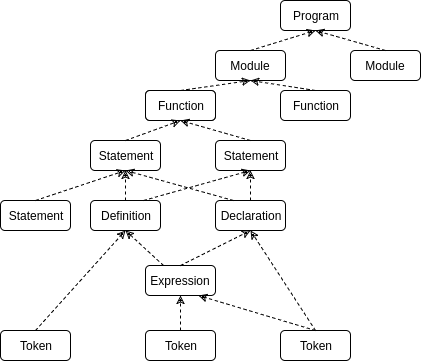
\includegraphics[width=0.45\textwidth]{software_layers}
	\caption{Software layers - shown are the hierarchical layer architecture of software, from the Function level to the bottom, an element can be a composition of multiple types of sub-elements or even itself}
	\medskip
	\label{fig:clf}
\end{figure}

Recently, a Neural Machine Translation tutorial \cite{Thang} for TensorFlow is released, which gives the reader the ability to build a competitive translation model from scratch. As machine translation of human language is largely improved and successful by employing deep neural network, it is a reasonable target to do the same thing for programming language because we've seen that character-level is capable of writing Linux kernel after learning the entire Linux base source code, as described in \cite{Karpathy}. We believe that our work can be a good foundation for a neural network-based programming language translation, which is a more sophisticated task. 

\section{Conclusion}
This work proposes an approach to learn the mapping between languages. By utilizing the alignment of files across languages, we can learn the alignment of tokens in an unsupervised manner, then we can learn the share embeddings between languages. The shared embeddings are able to bring the benefits to learn the semantic cross-lingually. We show that we can map most of the elements between languages accurately under a fine-grained manner. This can be served as a foundation for more complicated tasks, such as programming language translation. In the future, we want to collect more data in different languages to learn a shared embeddings, then we want to adopt the embeddings as a part of a neural network-based program translation for multiple languages. 



\begin{acks}
	
\end{acks}
